\documentclass[a4paper,11pt]{article}
	\usepackage[utf8]{inputenc}
	\usepackage[italian]{babel}
	\usepackage{hyperref}	%Consente l'inserimento di \url
	\usepackage{booktabs}	%Utilità di abbellimento tabelle
	\usepackage{longtable}
	\usepackage{tabularx}
	%\usepackage{widetable}
	\usepackage{array}
	\usepackage{listings}
	\usepackage{graphicx}
	\usepackage{caption}
	\usepackage{fancyhdr}
	\newenvironment{fixpic}{}{} % [1]
	\usepackage[a4paper,top=3cm,bottom=3cm,left=2.5cm,right=2.5cm]{geometry}
	%******
	\usepackage{makeidx}
	\usepackage{textcomp}
	\usepackage{multirow}
	\usepackage{rotfloat}
	\usepackage{lastpage}
	\usepackage{array}
	\usepackage{float}
	% *************************************
	% QUI CODICE PER \SUBSUBSUBSECTION
	\usepackage{titlesec}
	\titleclass{\subsubsubsection}{straight}[\subsection]
	
	\newcounter{subsubsubsection}[subsubsection]
	\renewcommand\thesubsubsubsection{\thesubsubsection.\arabic{subsubsubsection}}
	\renewcommand\theparagraph{\thesubsubsubsection.\arabic{paragraph}} % optional; useful if paragraphs are to be numbered
	
	\titleformat{\subsubsubsection}
	  {\normalfont\normalsize\bfseries}{\thesubsubsubsection}{1em}{}
	\titlespacing*{\subsubsubsection}
	{0pt}{3.25ex plus 1ex minus .2ex}{1.5ex plus .2ex}
	
	\makeatletter
	\renewcommand\paragraph{\@startsection{paragraph}{5}{\z@}%
	  {3.25ex \@plus1ex \@minus.2ex}%
	  {-1em}%
	  {\normalfont\normalsize\bfseries}}
	\renewcommand\subparagraph{\@startsection{subparagraph}{6}{\parindent}%
	  {3.25ex \@plus1ex \@minus .2ex}%
	  {-1em}%
	  {\normalfont\normalsize\bfseries}}
	\def\toclevel@subsubsubsection{4}
	\def\toclevel@paragraph{5}
	\def\toclevel@paragraph{6}
	\def\l@subsubsubsection{\@dottedtocline{4}{7em}{4em}}
	\def\l@paragraph{\@dottedtocline{5}{10em}{5em}}
	\def\l@subparagraph{\@dottedtocline{6}{14em}{6em}}
	\makeatother
	
	\setcounter{secnumdepth}{4}
	\setcounter{tocdepth}{4}
	%FINE \SUBSUBSUBSECTION
	%****************************************
	%STYLE PER INSERIMENTO DEL CODICE
	\lstdefinestyle{style1}{
	  belowcaptionskip=1\baselineskip,
	  breaklines=true,
	  frame=L,
	  xleftmargin=\parindent,
	  language=Pascal,
	  showstringspaces=false,
	  basicstyle=\footnotesize\ttfamily,
	  keywordstyle=\bfseries\color{blue},
	  commentstyle=\itshape\color{blue},
	  identifierstyle=\color{blue},
	  stringstyle=\color{orange},
	}
	
	\lstdefinestyle{style2}{
	  belowcaptionskip=1\baselineskip,
	  frame=L,
	  xleftmargin=\parindent,
	  language=C,
	  basicstyle=\footnotesize\ttfamily,
	  commentstyle=\itshape\color{blue},
	}
	\lstset{style=style1}
	
	%FINE STYLE INSERIMENTO CODICE
	%*****************************************
	\usepackage[default]{cantarell} %% Use option "defaultsans" to use cantarell as sans serif only
	\usepackage[T1]{fontenc}        %% for font
	\hypersetup{colorlinks, linkcolor=black, urlcolor=blue}
	\newcommand{\addglos}{\begin{scriptsize}{\textbf{\ped{G}}} \end{scriptsize}} 
	\pagestyle{fancy}
	\fancyhead{}
	\fancyfoot{}
	%\fancyhead[L]{
\includegraphics[scale=0.28]{team_not_found.jpeg}}
	\fancyhead[L]{
\includegraphics[scale=0.15]{../../team404_small.jpg} \hspace{2mm} QUIZZIPEDIA}
	\fancyhead[R]{\leftmark}
	\fancyfoot[L]{Universit\`a degli studi di Padova - IS 2015/2016 \\ \url{team404swe@gmail.com}}

	
	%Commando usato per la tabella di informazioni sul documento
	\newcommand{\introtab}[9]{
		\begin{table}[ht]
		\begin{center}		
		\begin{tabular}{r l}			
			\toprule		
			\multicolumn{2}{c}{\textbf{ Informazioni sul documento }} \\
			\midrule 
			\textbf{Nome Documento}			& \vline \hspace{3.5 mm} {#1} \\
			\textbf{Versione}				& \vline \hspace{3.5 mm} {#2} \\
			\textbf{Uso} 					& \vline \hspace{3.5 mm} {#3} \\
			\textbf{Data Creazione} 		& \vline \hspace{3.5 mm} {#4} \\
			\textbf{Data Ultima Modifica} 	& \vline \hspace{3.5 mm} {#5} \\
			\textbf{Redazione}				& \vline \hspace{3.5 mm} {#6} \\
											%& \vline \hspace{3.5 mm} {#7} \\	
			\textbf{Verifica} 				& \vline \hspace{3.5 mm} {#7}	\\
			\textbf{Approvazione}			& \vline \hspace{3.5 mm} {#8}\\	
			\textbf{Committente} 			& \vline \hspace{3.5 mm} Zucchetti SPA\\
			\textbf{Lista di distribuzione} & \vline \hspace{3.5 mm} Prof. Vardanega Tullio \\														& \vline \hspace{3.5 mm} TEAM404 \\
	\bottomrule	
	\end{tabular}
	\end{center}
	\end{table}
	}
	% Comando di inizio del registro
	\newcommand{\beginregistro}{
		%\begin{longtable}{{|p{0.10\textwidth}|p{0.20\textwidth}|p{0.15\textwidth}|p{0.50\textwidth}|}}
		\begin{longtable}{{|p{1.5cm}|p{2.5cm}|p{2cm}|p{8cm}|}} 
	 		\hline	
	}
	% commando usato pr inserire una riga al registro delle modifiche
	\newcommand{\rigaregistro}[4]{
		{\footnotesize #1} & {\footnotesize #2} &  {\footnotesize #3} &  {\footnotesize #4} \\
			\hline	
	}
	% Comando di fine registro
	\newcommand{\fineregistro}{ \end{longtable}	}
	
	%************************************************
	% commandi per il GLOSSARIO
	%***********************************************
	% Commando di inizio tabella Glossario
	\newcommand{\beginglos}{
		\begin{longtable}{{p{0.20\textwidth}p{0.65\textwidth}}}	
	}
	% Commando per i termini del glossario
	
	\newcommand{\itemglos}[2]{
		\textbf{#1 :} & {#2} \\ \\ \\
	}
	% Commando fine Glossario
	\newcommand{\fineglos}{ \end{longtable} }
	% Comando per aggiungere una ssezione numerata con lettere al glossario
	\newcommand{\sezione}{
	\subsection{}	
	\rule[0.3pt]{\linewidth}{0.4pt} \\ % Linea orizzontale
	}
	
\newcommand{\sezioneglos}[1] { 
  \newpage
  \cleardoublepage
  \phantomsection
  \addcontentsline{toc}{section}{#1}
  \vspace{11pt}
  \textbf{\huge{#1} } % Lettera grande 
  \\
  \rule[0.3pt]{\linewidth}{0.4pt} \\ % Linea orizzontale
  \fancyhead[R]{#1}
}
\usepackage[utf8]{inputenc}
\usepackage{hyperref}	%Consente l'inserimento di \url
\usepackage{booktabs}	%Utilità di abbellimento tabelle
\usepackage{caption}	%Caption tabelle
\usepackage{graphicx}   %Inserimento immagini
\usepackage{tabularx}	%tabelle migliorate
\usepackage{eurosym}	%Inserimento del simbolo €
\usepackage{geometry}	%Spostamento di elementi nella pagina
\hypersetup{colorlinks, linkcolor=black, urlcolor=blue}


\graphicspath{ {./Images/} }
\title{\textbf{{\fontsize{10mm}{6mm}\selectfont QUIZZIPEDIA}}}

\makeindex

\begin{document}
	\maketitle
	
	\begin{center}

	
\includegraphics{../../team_not_found.jpg}\\	
	\fontsize{5mm}{3mm}\url{team404swe@gmail.com}\\
	\vspace{40mm}
	\textbf{ Piano di Progetto 1.0}
	\end{center}
	\thispagestyle{empty}	% per togliere il numero in fondo pagina
	\introtab{Piano di Progetto}			%1 nome documento
			{1.0} 							%2 versione
			{Esterno} 						%3 Uso
			{21 dicembre 2015} 				%4 Data cre
			{\today} 						%5 Data mod
			{Davide Bortot}					%6 Redazione1
			%{} 								%7 Redazione2
			{Andrea Multineddu} 			%8 Verifica
			{Davide Bortot} 					%9 Approvazione
	
	\newpage
	\thispagestyle{empty}
	\null
	
	\newpage
	\fancyfoot[R]{\thepage}
	\pagenumbering{Roman}
	\section*{Registro delle modifiche}
		\begin{longtable}{{|p{0.10\textwidth}|p{0.15\textwidth}|p{0.15\textwidth}|p{0.50\textwidth}|}} 
	 		\hline			
			\rigaregistro{\textbf{Versione}}{\textbf{Autore}}{\textbf{Data}}{\hspace{5 mm} \textbf{Descrizione}}
			
			\rigaregistro{1.0}{D. Bortot \newline(Responsabile)}{15/03/2016}{Approvazione documento.}
			\rigaregistro{0.3}{A. Multineddu \newline(Verificatore)}{15/03/2016}{Revisione finale.}
			\rigaregistro{0.2.1}{D. Bortot \newline(Responsabile)}{14/03/2016}{Aggiustamenti minori alla formattazione del documento, correzione typo.}
			\rigaregistro{0.2}{A. Luca \newline(Verificatore)}{14/03/2016}{Revisione di stile. Segnalazione errori tipografici.}
			\rigaregistro{0.1.2}{D. Bortot \newline(Responsabile)}{06/03/2016}{Aggiustamento  dei capitoli 6 e 7, rivalutati su un preventivo minimo adeguato al gruppo da 6 elementi.}
			\rigaregistro{0.1.1}{D. Bortot \newline(Responsabile)}{22/01/2016}{Aggiustamento sezione 2.2}
			\rigaregistro{0.1}{A. Multineddu \newline(Verificatore)}{22/01/2016}{Prima revisione del documento, segnalato errore nella sezione 2.2}
			\rigaregistro{0.0.5}{D. Bortot \newline(Responsabile)}{18/01/2016}{Generazione e inserimento dei grafici relativi ai capitoli 6 e 7, e completamento di quest'ultimi.}
			\rigaregistro{0.0.4}{D. Bortot \newline(Responsabile)}{08/01/2016}{Completamento di testo e tabelle della "Pianificazione". Prima stesura del "Conto Economico Preventivo".}
			\rigaregistro{0.0.3}{D. Bortot \newline(Responsabile)}{03/01/2016}{Completamento "Analisi dei rischi". Primo abbozzo di "Pianificazione".}
			\rigaregistro{0.0.2}{D. Bortot \newline(Responsabile)}{28/12/2015}{Completamento "Introduzione". Redazione dei capitoli "Organizzazione" e "Analisi del ciclo di vita software". Primo abbozzo dell' "Analisi dei rischi".}
			\rigaregistro{0.0.1}{D. Bortot \newline(Responsabile)}{21/12/2015}{Prima stesura del documento. Prima redazione del paragrafo "Introduzione".}		
			\caption{Versionamento del documento} 
		\end{longtable}
		
	\newpage
	\tableofcontents
	
	\newpage
	\listoftables
	\listoffigures	
	
	\newpage
	\pagenumbering{arabic}
	\section{Sommario}
	Questo documento illustra il Piano di Progetto del gruppo \textbf{Team404} relativo al capitolato \textbf{Quizzipedia}, commissionato da \textbf{Zucchetti S.p.A.}
	\\
	Lo scopo del documento è definire e presentare al committente le scelte progettuali significative adottate (quali il modello di ciclo di vita scelto per lo sviluppo e la politica di gestione dei rischi adottata), le problematiche d'interesse incontrate durante l'avanzamento ed un'adeguata offerta tecnico-economica relativa al progetto.
	
	\newpage
	\section{Introduzione}
	\subsection{Scopo del documento}
	Nelle sezioni successive del presente documento, dopo una rapida visione d'insieme del prodotto che il gruppo \textbf{Team404} si prefigge di sviluppare, verrà presentato l'organigramma del gruppo e la definizione dei ruoli di progetto, relativa assegnazione dei ruoli e la pianificazione delle risorse , l'analisi dei rischi correlata ed il piano economico preventivo.
	\subsection{Scopo del prodotto}
	Il progetto \textbf{Quizzipedia} ha come obiettivo lo sviluppo di un sistema software basato su tecnologie Web (Javascript\addglos, Node.js\addglos, HTML5\addglos, CSS3\addglos) che permetta la creazione, gestione e fruizione di questionari. Il sistema dovrà quindi poter archiviare i questionari suddivisi per argomento, le cui domande dovranno essere raccolte attraverso uno specifico linguaggio di markup (Quiz Markup Language) d'ora in poi denominato QML\addglos. In un caso d'uso a titolo esemplificativo, un "esaminatore" dovrà poter costruire il proprio questionario scegliendo tra le domande archiviate, ed il questionario così composto sarà presentato e fruibile all' "esaminando", traducendo l'oggetto QML\addglos in una pagina HTML\addglos, tramite un'apposita interfaccia web. Il sistema presentato dovrà inoltre poter proporre questionari preconfezionati e valutare le risposte fornite dall'utente finale.
	\\
	Per un'analisi più approfondita del progetto si rimanda al documento "\textit{analisi\_dei\_requisiti\_1.0.pdf}".
	\subsection{Glossario}
	Viene allegato un glossario nel file ``\textit{glossario\_1.0.pdf}'' nel quale viene data una definizione a tutti i termini che in questo documento appaiono con il simbolo "\addglos" a pedice .
	\subsection{Riferimenti}
		\subsubsection{Normativi}
		\begin{itemize}
			\item Capitolato d'appalto Quizzipedia:\\
			\url{http://www.math.unipd.it/~tullio/IS-1/2015/Progetto/C5.pdf}
			\item Norme di Progetto: "\textit{norme\_di\_progetto\_1.0.pdf}"
		\end{itemize}
		\subsubsection{Informativi}
		\begin{itemize}
			\item Corso di Ingegneria del Software anno 2015/2016:\\
			\url{http://www.math.unipd.it/~tullio/IS-1/2015/}
			\item Regole del progetto didattico:\\
			\url{http://www.math.unipd.it/~tullio/IS-1/2015/Dispense/PD01.pdf}
			\url{http://www.math.unipd.it/~tullio/IS-1/2015/Progetto/}\\
			\url{http://www.math.unipd.it/~tullio/IS-1/2015/Progetto/PD01b.html}
		\end{itemize}
	\pagebreak
	
	\newpage
	\section{Organizzazione}	
	\subsection{Organigramma}
	\subsection*{Redazione}
	\begin{table}[h!]
		\begin{tabularx}{\textwidth}{XcX}
			\textbf{Nominativo} & \textbf{Data} &\hspace{20 mm}  \textbf{Firma}\\
			\midrule
			Davide Bortot & 18/01/2016 & \hspace{20 mm} 
\includegraphics[scale=0.35]{../Firme/db.jpg} \\
			\midrule
		\end{tabularx}
	\caption{Redazione documento}
	\end{table}

	\subsection*{Revisione}
	\begin{table}[h!]
		\begin{tabularx}{\textwidth}{XcX}
			\textbf{Nominativo} & \textbf{Data} &\hspace{20 mm}  \textbf{Firma}\\
			\midrule
			Andrea Multineddu & 15/03/2016 & \hspace{20 mm} 
\includegraphics[scale=0.3]{../Firme/multi.jpg} \\
			\bottomrule
		\end{tabularx}
	\caption{Revisione documento}
	\end{table}
	
	\subsection*{Approvazione}
	\begin{table}[h!]
		\begin{tabularx}{\textwidth}{XcX}
			\textbf{Nominativo} & \textbf{Data} &\hspace{20 mm}  \textbf{Firma}\\
			\midrule
			Davide Bortot & 15/03/2016 & \hspace{20 mm} 
\includegraphics[scale=0.35]{../Firme/db.jpg} \\ 
			\bottomrule
		\end{tabularx}
	\caption{Approvazione documento}
	\end{table}

	\subsection*{Accettazione dei componenti}
	\begin{table}[h!]
		\begin{tabularx}{\textwidth}{XcX}
			\textbf{Nominativo} & \textbf{Data} &\hspace{20 mm}  \textbf{Firma}\\
			\midrule
			Davide Bortot & 18/01/2016 & \hspace{20 mm} 
\includegraphics[scale=0.3]{../Firme/db.jpg}\\	
				Martin Vadice Mbouenda & 08/03/2016 & \hspace{20 mm} 
\includegraphics[scale=0.35]{../Firme/martin.png} \\ 
				Marco Crivellaro & 10/03/2016 &\hspace{20 mm} 
\includegraphics[scale=0.3]{../Firme/crivellaro.png} \\ 
				Alex Beccaro & 08/03/2016 & \hspace{20 mm} 
\includegraphics[scale=0.3]{../Firme/becks.jpg} \\ 
				Luca Alessio & 10/03/2016 & \hspace{20 mm} 
\includegraphics[scale=0.3]{../Firme/alessio.jpg} \\ 
				Andrea Multineddu & 10/03/2016 & \hspace{20 mm} 
\includegraphics[scale=0.3]{../Firme/multi.jpg} \\ 
			\bottomrule
		\end{tabularx}
	\caption{Accettazione dei componenti}
	\end{table}
		\newpage
	\subsubsection*{Componenti}
			\begin{table}[h!]			
				\begin{center}
				\begin{tabular}{l c l}
				\textbf{Nominativo} & \textbf{Matricola} & \textbf{Posta elettronica}\\
				\midrule
				Davide Bortot & 1070213 & davide.bortot94@gmail.com \\
				Martin Vadice Mbouenda & 601901 & tinovad@hotmail.com \\
				Marco Crivellaro & 544339 & marcocrivellaro0603@gmail.com \\
				Alex Beccaro & 1072686 & alex.becks@hotmail.it \\
				Luca Alessio & 1070690 & lucaalessio1994@gmail.com \\
				Andrea Multineddu & 1049261 & andrea.multineddu@gmail.com \\
				\midrule
				\end{tabular}
			\end{center}
			\caption{Componenti}
			\end{table}	

	\subsection{Ruoli di progetto}
		Per un più sistematico sviluppo di progetto, e per adempiere alle regole di progetto riportate nella sezione Riferimenti, ai componenti del gruppo verranno assegnati nel tempo 6 diversi ruoli, così definiti:
		\begin{itemize}
			\item \textbf{Responsabile: }È il responsabile ultimo, per conto del suo gruppo, dei risultati del progetto.
Elabora ed emana piani e scadenze, ed approva l'emissione di documenti. 
Coordina le attività del gruppo, relazionandosi con il controllo di qualità interno al progetto. 
Redige Organigramma e Piano di Progetto, ed approva inoltre l'Offerta ed i relativi allegati;
			\item \textbf{Amministratore: }È responsabile dell'efficienza e dell'operatività dell'ambiente di sviluppo, della redazione e attuazione di piani e procedure di gestione per la qualità.
Controlla versioni e configurazioni del prodotto e gestisce l'archivio della documentazione di progetto. 
Collabora alla redazione del Piano di Progetto e nel contempo redige le Norme di Progetto per conto del Responsabile;
			\item \textbf{Analista: }È responsabile delle attività di analisi. 
Redige lo Studio di Fattibilità (documento interno al gruppo) e l'Analisi dei Requisiti;
			\item \textbf{Progettista: }È responsabile delle attività di progettazione. 
Redige Specifica Tecnica, Definizione di Prodotto e la parte programmatica del Piano di Qualifica;
			\item \textbf{Programmatore: }È responsabile delle attività di codifica miranti alla realizzazione del prodotto e delle componenti di ausilio necessarie per l'esecuzione delle prove di verifica e validazione;
			\item \textbf{Verificatore: }È responsabile delle attività di verifica.
Redige la parte retrospettiva del Piano di Qualifica che illustra l'esito e la completezza delle verifiche e delle prove effettuate secondo il piano.
		\end{itemize}
	\pagebreak	
	
	\newpage
	\section{Analisi del ciclo di vita software}	
	In questo capitolo vengono presentati i principali modelli di ciclo di vita applicabili allo sviluppo di un progetto software, e viene in seguito spiegata la scelta del modello che il gruppo \textbf{Team404} ha deciso di adottare per \textbf{Quizzipedia}.
	\subsection{Modelli di cicli di vita}
	\subsubsection{Modello Iterativo}
	I modelli iterativi prevedono che lo sviluppo proceda in fasi sequenziali e ben distinte da condizioni d'entrata e d'uscita, ammettendo però che errori ed imprevisti nel percorso (quale la variazione dei requisiti del sistema) riportino lo sviluppo ad uno stadio precedente per applicare le correzioni/migliorie necessarie. Queste caratteristiche rendono il modello adatto a progetti in cui errori di progettazione e analisi, o variazioni dei requisiti, sono molto probabili, consentendo di mantenere maggior parte del lavoro fatto e di ripartire prontamente da uno stato d'integrità noto del sistema. Come s'intuisce il modello non ha però sicurezza di convergenza, e rischia quindi di estendere negativamente i tempi di sviluppo.
	\subsubsection{Modello Incrementale}
	Il modello incrementale è un raffinamento del modello iterativo. Lo sviluppo procede per rilasci multipli e successivi, ciascuno dei quali realizza un incremento di funzionalità. L'analisi dei requisiti e la progettazione architetturale vengono eseguite solamente una volta all'inizio, identificando e fissando così univocamente i requisiti di base del progetto. Si avanza poi tramite cicli incrementali, procedendo a soddisfare prima i requisiti essenziali, e poi quelli opzionali e desiderabili. Ogni ciclo viene decomposto in:
	\begin{enumerate}
	\item Sviluppo dell'incremento di sistema;
	\item Validazione dell'incremento;
	\item Integrazione dell'incremento;
	\item Validazione del sistema.
	\end{enumerate}
	Così facendo alla fine di ogni ciclo il sistema è sempre in uno stato consistente, ed ogni incremento aggiunge valore al sistema. Il modello incrementale è quindi adatto a progetti in cui i requisiti fondamentali sono ben definiti, così da formare una solida struttura di base alla quale aggiungere incrementalmente funzionalità.
	\subsubsection{Modello Evolutivo}
	Il modello evolutivo prevede il riattraversamento di più fasi del ciclo di vita e la generazione di più versioni di sviluppo parallele. Questo lo rende adatto in situazioni in cui ci si aspetta che il sistema dovrà rispondere a bisogni non inizialmente preventivabili. Evidentemente il modello comporta anche un notevole dispendio di risorse.
	\subsubsection{Modello a Spirale}
	Il  modello a spirale pone l'accento sull'analisi dei rischi e sullo stretto rapporto col committente nel definire chiaramente obiettivi, pianificazioni e gestione dei rischi; all'analisi viene solitamente affiancato lo sviluppo di prototipi. Il modello è applicabile quindi a progetti in cui la componente del rischio è particolarmente presente ed impattante.
	\subsection{Scelta del modello}
	Il modello di ciclo di sviluppo (non sarà un ciclo di vita, mancando la parte di manutenzione) scelto per \textbf{Quizzipedia} è il modello Incrementale; essendo infatti il capitolato d'appalto ben strutturato e i requisiti essenziali ben specificati, è ragionevole definire nelle prima fasi del progetto una struttura di base alla quale aggiungere incrementalmente funzionalità nei momenti successivi dello sviluppo. Il modello adottato inoltre garantisce una decente convergenza e un avanzamento continuo, riducendo il rischio di ritardi di consegna, o peggio ancora la mancata partecipazione ad una revisione.
	\newpage
	\section{Analisi dei rischi}
	In questo capitolo verranno valutati i rischi e gli impedimenti che possono insorgere durante l'intera durata dello sviluppo del progetto. Per meglio strutturare e comprendere il problema a ogni rischio verranno associate:
	\begin{itemize}
	\item \textbf{Descrizione:} descrizione testuale del problema in analisi.
	\item \textbf{Probabilità:} una stima probabilistica che il problema si presenti, valutata in una scala da 1 a 3, dove 3 è il massimo.
	\item \textbf{Impatto:} l'influenza negativa che avrebbe il presentarsi del problema in analisi, valutato con una scala a tre livelli (A, B, C) dove:
	\begin{itemize}
		\item \textbf{A)} problema poco impattante e facilmente risolvibile;
		\item \textbf{B)} problema impattante ma risolvibile con soluzioni adeguate;
		\item \textbf{C)} problema molto impattante e difficilmente risolvibile.
	\end{itemize}
	\end{itemize}
	Inoltre verrà suggerita per ogni rischio una strategia indicata a ridurne l'impatto, ove possibile, e nel caso il problema si sia già presentato verrà riportata la soluzione effettivamente adottata dal gruppo.
	\subsection{Risorse Umane}
		\subsubsection{Incompatibilità componenti del gruppo}
		Rappresenta la possibilità che tra i componenti del gruppo sorgano incongruenze tali da impedire il corretto avanzamento del progetto.
		\begin{itemize}
		\item \textbf{Probabilità:} 1
		\item \textbf{Impatto:} B
		\end{itemize}
		Fino al momento della stesura del presente documento, il gruppo è stato coeso e propenso a trovare facilmente strategie e idee di comune accordo. Nel caso il problema si verificasse sarà necessario l'intervento di un'autorità maggiore (prima fra tutte il Responsabile di progetto) che appiani le divergenze. Nel caso le controversie persistano è valutabile l'opzione di estromettere dal gruppo l'elemento più problematico.
		\subsubsection{Impegni esterni al progetto didattico}
		Rappresenta la possibilità che alcuni elementi del gruppo non riescano ad adempiere ai propri doveri progettuali a causa di impegni personali o universitari.
		\begin{itemize}
		\item \textbf{Probabilità:} 2
		\item \textbf{Impatto:} B
		\end{itemize}
		Questo tipo di problema è stimabile ed evitabile fin dall'inizio del progetto tramite una dichiarazione, anche informale, dei propri obiettivi ed impegni da parte di tutti i componenti del gruppo. Così facendo si possono adeguatamente preventivare le ore di lavoro necessarie venendo incontro ad alle esigenze personali. Nel caso di eventi/impegni inaspettati la scelta più ovvia è un'immediata redistribuzione delle ore individuali in modo da garantire il completamento efficiente dei compiti.
		\subsubsection{Indisponibilità prolungata}
		Rappresenta la possibilità che qualche elemento, per ragioni inaspettate, si ritrovi impossibilitato a partecipare attivamente allo sviluppo del progetto per un lasso di tempo prolungato. 
		\begin{itemize}
		\item \textbf{Probabilità: }1
		\item \textbf{Impatto: }C
		\end{itemize}
		Questo problema, seppur poco probabile, è particolarmente impattante e difficile da mitigare. Prima di tutto va valutata la possibilità di accollare tutto il lavoro dell'elemento indisposto ai compagni; in caso non sia possibile, il progetto subirà un'inevitabile ritardo.
	\subsection{Conoscenze e Strumenti}
		\subsubsection{Carenza di conoscenze tecniche}
		Rappresenta la possibilità che uno o più componenti del gruppo non dispongano delle conoscenze tecniche necessarie ad utilizzare proficuamente le tecnologie e gli strumenti di progetto.
		\begin{itemize}
		\item \textbf{Probabilità: }3
		\item \textbf{Impatto: }A
		\end{itemize}
		La maggior parte delle conoscenze necessarie è nota fin dall'inizio del progetto, quindi per ridurre l'impatto è sufficiente preventivare alcune ore di formazione individuale tese ad appianare le carenze evidenziate.
		\subsubsection{Carenza di strumenti adeguati}
		Rappresenta la possibilità che il progetto non possa proseguire, o venga pesantemente rallentato, a causa della mancanza (o utilizzo scorretto) degli strumenti di supporto allo sviluppo.
		\begin{itemize}
		\item \textbf{Probabilità: }1
		\item \textbf{Impatto: }B
		\end{itemize}
		Al verificarsi del problema è necessario agire tempestivamente ricercando strumenti alternativi minimizzando la perdita del lavoro già fatto. Nel caso di utilizzo scorretto, si rimanda alla sezione 5.2.1.
	\subsection{Errori d'analisi}
		\subsubsection{Errore in fase di analisi dei requisiti}
		Rappresenta la possibilità che i requisiti rilevati durante la fase di analisi dei requisiti siano errati o insufficienti a definire adeguatamente il sistema che si andrà a sviluppare.
		\begin{itemize}
		\item \textbf{Probabilità:} 2
		\item \textbf{Impatto:} B
		\end{itemize}
		La gravità del problema è maggiore quanto più tardi nello sviluppo si presenta. E' normale ed auspicabile che durante le prime parti dello sviluppo il numero dei requisiti continui ad aumentare. E' però necessario che prima di iniziare la progettazione architetturale del prodotto la maggior parte dei requisiti sia analizzata e confermata. Requisiti che emergessero in fasi più avanzate di sviluppo comporterebbero ore di lavoro straordinarie per definire ed integrare il nuovo requisito nel sistema. Per assicurare una miglior completezza ed un lavoro di maggior qualità, più componenti hanno lavorato contemporaneamente all' analisi dei requisiti nella prima fase del progetto.
		\subsubsection{Errore in fase di studio di fattibilità}
		Rappresenta la possibilità che lo studio di fattibilità contenga considerazioni particolarmente errate.
		\begin{itemize}
		\item \textbf{Probabilità:} 1
		\item \textbf{Impatto:} A
		\end{itemize}
		Eventuali mancanze non preventivate nello studio di fattibilità vanno immediatamente documentate e risolte il prima possibile.
		\subsubsection{Errore di stima risorse/costi}
		Rappresenta la possibilità che, nella fase di analisi iniziale, la pianificazione sia basata su di un'errata valutazione delle risorse necessarie e dei costi correlati.
		\begin{itemize}
		\item \textbf{Probabilità:} 2
		\item \textbf{Impatto:} B
		\end{itemize}
		A seconda dell'importanza dell'errore, è necessario un tempestivo aggiornamento della pianificazione e un'adatta redistribuzione delle ore di lavoro, con conseguente aggiustamento del consuntivo. È necessario che la pianificazione venga più volte controllata e validata per evitare tali complicazioni future.
	\subsection{Ritardi}
		\subsubsection{Ritardo nel completamento di un'attività}
		Rappresenta il rischio che un'attività importante non venga completata nella data prefissata, causando potenziali ritardi in altre attività dipendenti dalla stessa.
		\begin{itemize}
		\item \textbf{Probabilità:2}
		\item \textbf{Impatto:} B
		\end{itemize}
		Nonostante non sia auspicabile è possibile che un evento del genere accada. È essenziale quindi che, attraverso un attento controllo dei tempi di progetto, il responsabile dell'attività comunichi prima della data di scadenza che  il task\addglos sta procedendo a rilento, chiedendo risorse aggiuntive per colmare il ritardo. Se il ritardo fosse incolmabile sarà necessario procedere ad una revisione della pianificazione che permetta di rispettare le scadenze.
		\subsubsection{Ritardata partecipazione ad una revisione}							Rappresenta il rischio che per un sommarsi dei problemi sopra elencati il gruppo non possa partecipare ad una revisione nelle date prefissate.
		\begin{itemize}
		\item \textbf{Probabilità:} 1
		\item \textbf{Impatto:} C
		\end{itemize}
		Tale rischio non è risolvibile, ma obbliga il gruppo a far slittare la propria pianificazione alla data di revisione successiva. Nel caso di un evento così impattante è necessario individuare esattamente i fattori che lo hanno causato e prendere tutte le contromisure necessarie in modo che non possa verificarsi nuovamente alla revisioni successive. Il gruppo \textbf{Team404} ha tutti gli interessi e le intenzioni a non permettere che tale rischio si avveri, imprescindibilmente dagli eventi.
	\pagebreak	
		
	\newpage
	\section{Pianificazione delle risorse}	
	Questa sezione è dedicata all'analisi e distribuzione delle risorse necessarie durante l'intera durata dello sviluppo. Verranno di seguito riportate la scadenze da rispettare per il progetto didattico. Successivamente verranno precisate la suddivisione e rotazione dei ruoli, correlate dal numero di ore dedicato ad ogni attività, nel succedersi delle fasi di sviluppo del progetto. I costi della pianificazione così proposta verranno poi riassunti nel Conto Economico Preventivo.
	\subsection{Scadenze}
	Le Scadenze, cioè le date di revisione, alle quali il gruppo \textbf{Team404} si prefigge di partecipare sono le seguenti:
	\begin{table}[h!]
	\begin{center}
		\begin{tabularx}{240pt}{Xc}
			\textbf{Scadenza} & \textbf{Data}\\
			\midrule
			Revisione dei Requisiti & 18/04/2016\\
			Revisione di Progettazione & 23/05/2016\\
			Revisione di Qualifica & 17/06/2016\\
			Revisione di Accettazione & 11/07/2016\\
			\bottomrule
		\end{tabularx}
	\end{center}
	\caption{Scadenze ufficiali	}
	\end{table}
	
	\subsection{Pianificazione attività di sviluppo}
	Basandosi sulle scadenze riportate si è deciso di suddividere la pianificazione in più parti, ognuna identificata dallo spazio temporale tra un revisione e l'altra. Definita la rotazione dei ruoli, per ogni fase verranno fissate le ore/persona che ognuno dovrà ricoprire nel proprio ruolo.
	 \subsubsection{Rotazione dei ruoli}
I ruoli subiranno una rotazione per permettere a tutti gli elementi di avere esperienza dei vari processi che compongono lo sviluppo di un progetto software complesso. Durante le varie fasi del progetto è possibile, ed auspicabile, che alcuni ruoli non vengano ricoperti da nessun elemento del gruppo, e che un ruolo venga invece ricoperto da più persone. Ad esclusione dell'analisi iniziale, la durata media dei periodi individuati è di un mese; si è quindi deciso di attuare la rotazione dei ruoli circa ogni due settimane, dal momento che una rotazione più dinamica inibirebbe la produttività dei singoli elementi.
		\pagebreak
		\subsubsection{Analisi}
		L'analisi iniziale ha avuto inizio il 20/12/2015 ed è finita il 17/04/2016. Il buon svolgimento di questa fase è prerequisito essenziale per procedere efficientemente alla successiva fase di progettazione. Durante questo periodo il gruppo ha posto la propria attenzione sui seguenti punti:
		\begin{itemize}
		\item Produrre un'attenta analisi dei requisiti che descriva il più fedelmente possibile le esigenze del prodotto;
		\item Stabilire una pianificazione ragionevole delle fasi di progetto;
		\item Definire l'insieme delle norme di progetto e gli obiettivi di qualità da conseguire;
		\item Verificare, correggere e validare il lavoro svolto.
		\end{itemize}
		Le attività sono state svolte secondo rotazione di ruoli riportata in tabella:
		\begin{table}[h!]			
		\begin{center}
			\begin{tabular}{l c c}
			\textbf{Componente} & \textbf{Ruolo I} & \textbf{Ruolo II} \\
			\midrule
			Davide Bortot & Responsabile & Amministratore\\
			Martin Vadice Mbouenda & Amministratore & Analista\\
			Marco Crivellaro & Analista & Verificatore\\
			Alex Beccaro & Analista & Responsabile\\
			Luca Alessio & Analista & Verificatore\\
			Andrea Multineddu & Verificatore & Analista\\
			\midrule
			\end{tabular}
		\end{center}
		\caption{Ruoli Analisi Iniziale}
		\end{table}
		
		La tabelle successive riportano la suddivisione in ore attuata per ogni ruolo e persona:
		\begin{table}[h!]			
		\begin{center}
			\begin{tabular}{l c c c}
			\textbf{Componente} & \textbf{Ore Ruolo I} & \textbf{Ore Ruolo II} & \textbf{Totale Ore}\\
			\midrule
			Davide Bortot & 15 & 8 & 23\\
			Martin Vadice Mbouenda & 17 & 5 & 22\\
			Marco Crivellaro & 15 & 9 & 24 \\
			Alex Beccaro & 19 & 6 & 25\\
			Luca Alessio & 13 & 8 & 21\\
			Andrea Multineddu & 18 & 4 & 22\\
			\midrule
			\textbf{Ore medie per persona} & & & \textbf{22.8}\\
			\end{tabular}
		\end{center}
		\caption{Ore/persona Analisi Iniziale}
		\end{table}
		\begin{table}[h!]			
		\begin{center}
			\begin{tabular}{l c}
			\textbf{Ruolo} & \textbf{Ore Totali} \\
			\midrule
			Analista & 56\\
			Verificatore & 35\\
			Amministratore & 25 \\
			Responsabile & 21\\
			\midrule
			\textbf{Totale} & \textbf{136}\\
			\end{tabular}
		\end{center}
		\caption{Ore/ruolo Analisi Iniziale}
		\end{table}
		\begin{figure}[h!]
		    \centering
			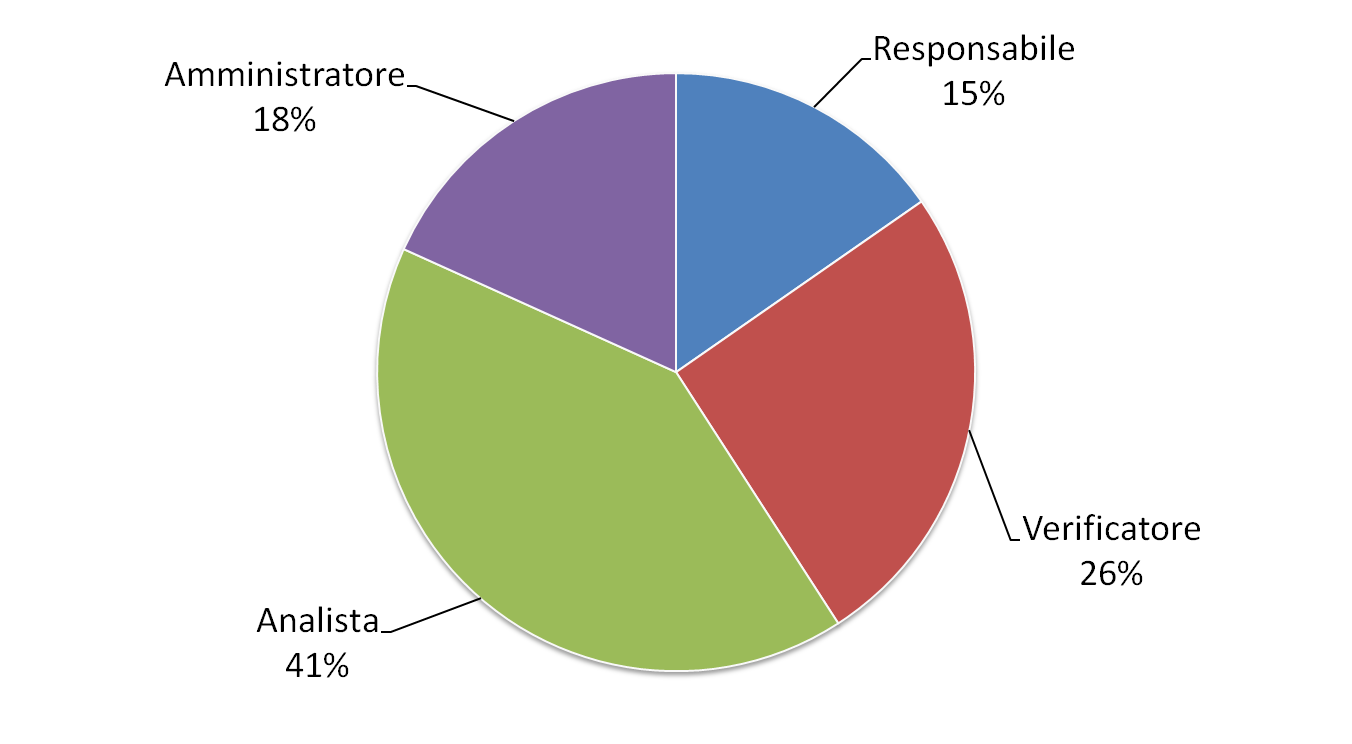
\includegraphics[scale=0.55]{../Images/pie_chart-Analisi_Iniziale}
			\caption{Incisione Ruoli Analisi Iniziale}
		\end{figure}
		
		Come evidenziato dalla Figura 1 la maggior parte dell'impegno è stata riposta nell'assicurare un'approfondita analisi dei requisiti, mentre c'è stato pari impegno nella stesura dei documenti di competenza rispettivamente di Responsabile e Amministratore. Più di un quarto delle ore preventivate è stato usato nel processo di verifica, controllo di qualità e validazione del materiale prodotto, processo che è continuato fino alla data di consegna. I costi sostenuti e le ore svolte in questa prima fase non verranno acclusi al preventivo, ma vengono riportati per completezza.
		\pagebreak
		\subsubsection{Progettazione}
		Questa fase avrà inizio il 19/04/2016 e finirà il 22/05/2016. In virtù dell'attenta analisi dei requisiti derivante dalla fase precedente, il gruppo conta di poter iniziare fin da subito un efficace attività di progettazione. In questo periodo lo sviluppo sarà centrato sui seguenti punti:
		\begin{itemize}
		\item Continuo raffinamento e validazione dei requisiti;
		\item Trasformazione dei requisiti in una solida progettazione architetturale, che costituisca una base il più possibile stabile per futuri incrementi;
		\item Traduzione della progettazione architetturale in progettazione di dettaglio, input concreto per la successiva fase di codifica;
		\item Verificare, correggere e validare il lavoro svolto.
		\end{itemize}
		Le attività si svolgeranno in linea di massima secondo la rotazione di ruoli riportata in Tabella 11. Per garantire a tutti gli elementi di partecipare nel ruolo di progettisti, ruolo principale della fase, alcuni elementi dovranno ricoprire più ruoli contemporaneamente.
		\begin{table}[h!]			
		\begin{center}
			\begin{tabular}{l c c}
			\textbf{Componente} & \textbf{Ruolo I} & \textbf{Ruolo II} \\
			\midrule
			Davide Bortot & Responsabile/Progett & Analista/Ver\\
			Martin Vadice Mbouenda & Analista/Ver & Responsabile/Progett\\
			Marco Crivellaro & Analista/Ver & Progettista\\
			Alex Beccaro & Progettista & Analista/Ver\\
			Luca Alessio & Progettista/Amm & Analista/Ver\\
			Andrea Multineddu & Analista/Ver & Progettista/Amm\\
			\midrule
			\end{tabular}
		\end{center}
		\caption{Ruoli Progettazione}
		\end{table}
		\pagebreak
		
		Le tabelle successive riportano la suddivisione in ore attuata per ogni ruolo e persona:
		\begin{table}[h!]			
		\begin{center}
			\begin{tabular}{l c c c}
			\textbf{Componente} & \textbf{Ore Ruolo I} & \textbf{Ore Ruolo II} & \textbf{Totale Ore}\\
			\midrule
			Davide Bortot & 10/18 & 5/15 & 48\\
			Martin Vadice Mbouenda & 5/14 & 5/18 & 42\\
			Marco Crivellaro & 5/15 & 20 & 40 \\
			Alex Beccaro & 20 & 5/15 & 40\\
			Luca Alessio & 18/5 & 5/15 & 43\\
			Andrea Multineddu & 5/15 & 18/10 & 48\\
			\midrule
			\textbf{Ore medie per persona} & & & \textbf{43,5}\\
			\end{tabular}
		\end{center}
		\caption{Ore/persona Progettazione}
		\end{table}
		\begin{table}[h!]			
		\begin{center}
			\begin{tabular}{l c}
			\textbf{Ruolo} & \textbf{Ore Totali} \\
			\midrule
			Progettista & 112 \\
			Verificatore & 89 \\
			Analista & 30\\
			Amministratore & 15\\
			Responsabile & 15\\
			\midrule
			\textbf{Totale} & \textbf{261}\\
			\end{tabular}
		\end{center}
		\caption{Ore/ruolo Progettazione}
		\end{table}
		\begin{figure}[h!]
		    \centering
			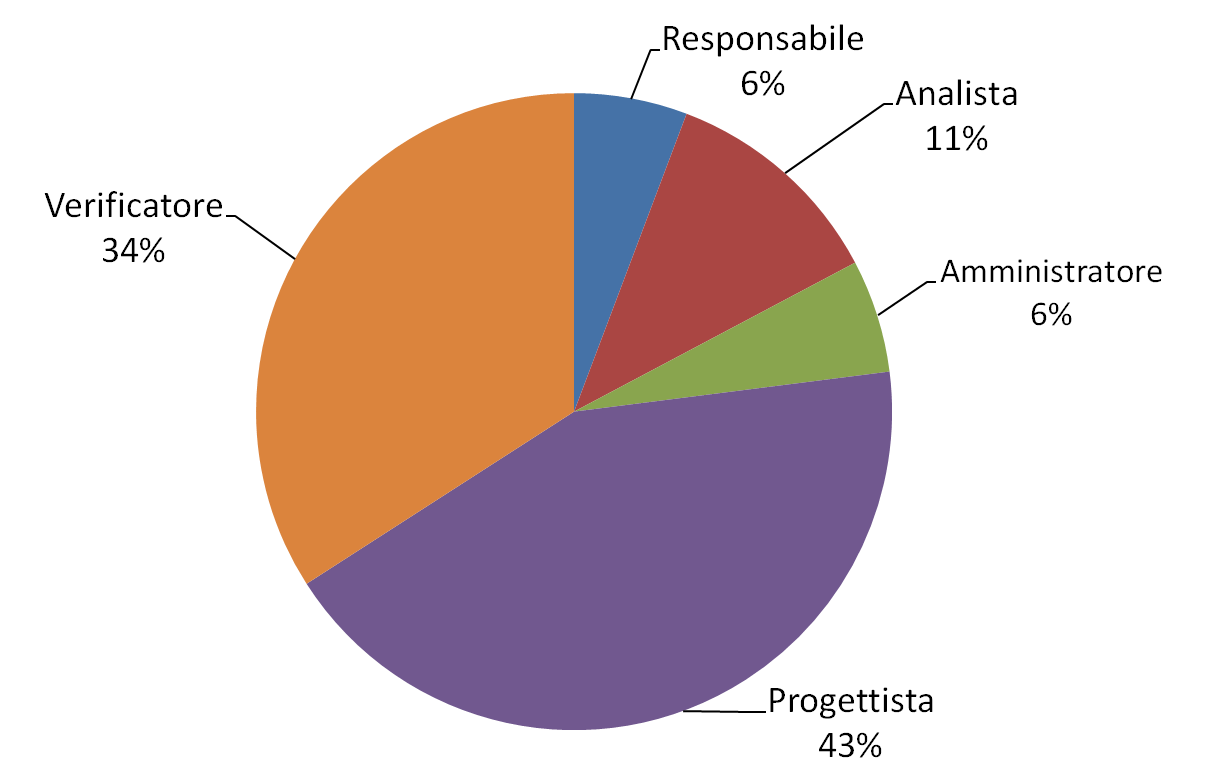
\includegraphics[scale=0.6]{../Images/pie_chart-Progettazione}
			\caption{Incisione Ruoli Progettazione}
		\end{figure}
		
		La suddivisione del lavoro è stata pensata in modo che l'attività del progettista, ruolo che tutti gli elementi ricopriranno almeno una volta durante la fase, sia controllata e supportata da una notevole quantità d'ore dedicate al processo di verifica. Questa è la fase alla quale vengono dedicate più ore in tutto il progetto, in modo da garantire una progettazione completa che permetta di iniziare la codifica senza bisogno di molti aggiustamenti ulteriori.
		\newpage
		\subsubsection{Codifica}
		Questa fase inizierà il 24/05/2016 e finirà il 16/06/2016. Nel primo periodo vi saranno le ultime attività di perfezionamento e correzione della progettazione; nel contempo inizierà l'attività di codifica basata sulla progettazione di dettaglio prodotta. Come per la fase precedente il processo principale, in questo caso la codifica, sarà continuamente monitorata e validata dal processo di verifica. Nell'ottica di consentire a tutto il gruppo di essere partecipe nel ruolo di Programmatore la rotazione dei ruoli è stata così definita:
		\begin{table}[h!]			
		\begin{center}
			\begin{tabular}{l c c}
			\textbf{Componente} & \textbf{Ruolo I} & \textbf{Ruolo II} \\
			\midrule
			Davide Bortot & Progettista/Ver & Programmatore\\
			Martin Vadice Mbouenda & Programmatore & Progettista/Ver\\
			Marco Crivellaro & Resp/Programm & Verificatore/Amm\\
			Alex Beccaro & Verificatore/Amm & Resp/Programm\\
			Luca Alessio & Programmatore  & Progettista/Ver\\
			Andrea Multineddu & Progettista/Ver & Programmatore\\
			\midrule
			\end{tabular}
		\end{center}
		\caption{Ruoli Codifica}
		\end{table}
		
		Le tabelle successive riportano la suddivisione in ore attuata per ogni ruolo e persona.
		\begin{table}[h!]			
		\begin{center}
			\begin{tabular}{l c c c}
			\textbf{Componente} & \textbf{Ore Ruolo I} & \textbf{Ore Ruolo II} & \textbf{Totale Ore}\\
			\midrule
			Davide Bortot & 5/10 & 20 & 35\\
			Martin Vadice Mbouenda & 18 & 5/10 & 33\\
			Marco Crivellaro & 10/18 & 10/5 & 43 \\
			Alex Beccaro & 10/10 & 5/20 & 45\\
			Luca Alessio & 20 & 10/10 & 40\\
			Andrea Multineddu & 5/10 & 22 & 37\\
			\midrule
			\textbf{Ore medie per persona} & & & \textbf{39}\\
			\end{tabular}
		\end{center}
		\caption{Ore/persona Codifica}
		\end{table}
		\begin{table}[h!]			
		\begin{center}
			\begin{tabular}{l c}
			\textbf{Ruolo} & \textbf{Ore Totali} \\
			\midrule
			Programmatore & 118 \\
			Verificatore & 60\\
			Progettista & 25 \\		
			Responsabile & 15\\
			Amministratore & 15 \\
			\midrule
			\textbf{Totale} & \textbf{233}\\
			\end{tabular}
		\end{center}
		\caption{Ore/ruolo Codifica}
		\end{table}
		
		\begin{figure}[h!]
		    \centering
			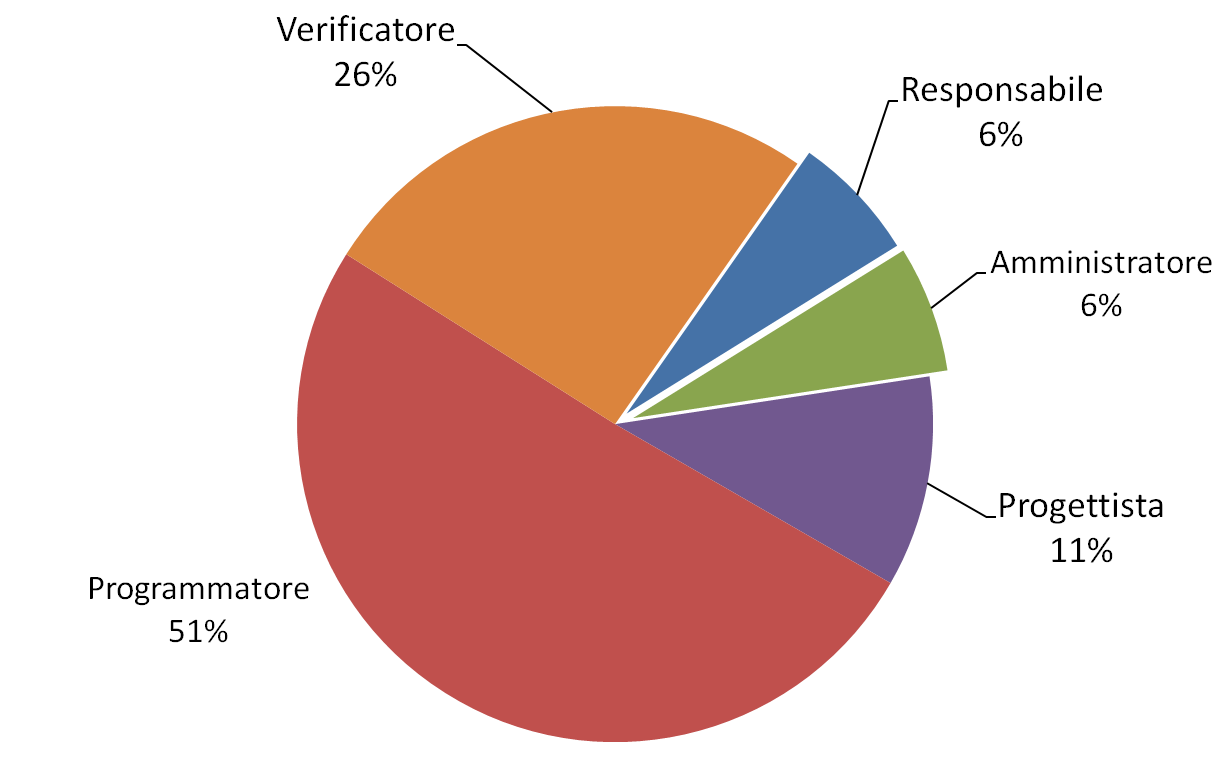
\includegraphics[scale=0.65]{../Images/pie_chart-Codifica}
			\caption{Incisione Ruoli Codifica}
		\end{figure}
		\clearpage
			
		\subsubsection{Verifica e validazione}
		Questa fase inizierà il 18/06/2016 e finirà l' 11/07/2016, in concomitanza con la Revisione di Accettazione. Scopo di quest'ultima fase è procedere ad un'attenta verifica e validazione del software prodotto, integrato in tutte le sue parti, ed al collaudo dell'intero sistema. L'ultima rotazione dei ruoli è stata decisa come in Tabella 17, con l'obiettivo di far partecipe l'intero gruppo del processo di verifica.
		\begin{table}[h!]			
		\begin{center}
			\begin{tabular}{l c c}
			\textbf{Componente} & \textbf{Ruolo I} & \textbf{Ruolo II} \\
			\midrule
			Davide Bortot & Programmatore & Amm/Verificatore\\
			Martin Vadice Mbouenda & Amm/Progettista & Verificatore\\
			Marco Crivellaro & Programmatore & Verificatore\\
			Alex Beccaro & Verificatore & Progettista\\
			Luca Alessio & Verificatore & Resp/Progettista\\
			Andrea Multineddu & Resp/Progettista & Verificatore\\
			\midrule
			\end{tabular}
		\end{center}
		\caption{Ruoli Verifica e Validazione}
		\end{table}
		\begin{table}[h]			
		\begin{center}
			\begin{tabular}{l c c c}
			\textbf{Componente} & \textbf{Ore Ruolo I} & \textbf{Ore Ruolo II} & \textbf{Totale Ore}\\
			\midrule
			Davide Bortot & 5 & 5/10 & 20\\
			Martin Vadice Mbouenda & 10/3 & 10 & 23\\
			Marco Crivellaro & 5 & 15 & 20 \\
			Alex Beccaro & 13 & 5 & 18\\
			Luca Alessio & 5 & 10/5 & 20\\
			Andrea Multineddu & 5/5 & 8 & 18\\
			\midrule
			\textbf{Ore medie per persona} & & & \textbf{20}\\
			\end{tabular}
		\end{center}
		\caption{Ore/persona Verifica e Validazione}
		\end{table}
		
		\begin{table}[h!]			
		\begin{center}
			\begin{tabular}{l c}
			\textbf{Ruolo} & \textbf{Ore Totali} \\
			\midrule
			Verificatore & 61\\
			Programmatore & 15 \\
			Progettista & 13 \\
			Amministratore & 15 \\
			Responsabile & 15\\
			\midrule
			\textbf{Totale} & \textbf{119}\\
			\end{tabular}
		\end{center}
		\caption{Ore/ruolo Verifica e Validazione}
		\end{table}
		
		\begin{figure}[h!]
		    \centering
			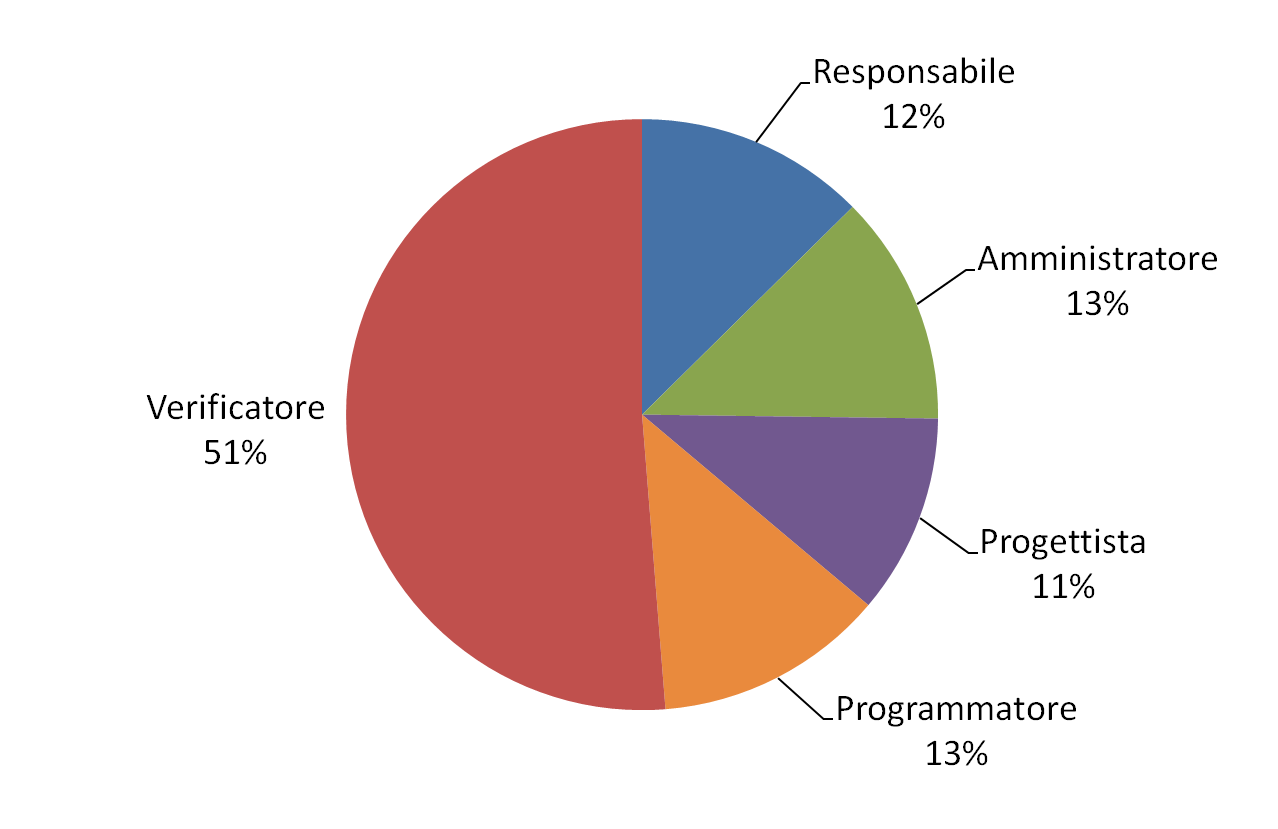
\includegraphics[scale=0.6]{../Images/pie_chart-V&V}
			\caption{Incisione Ruoli Verifica e Validazione}
		\end{figure}
		
	\newpage
	\section{Conto Economico Preventivo}
	\subsection{Vincoli economici e didattici}
	Come da regolamento del progetto didattico il costo minimo preventivato non dev'essere inferiore a 13.000,00 \euro. Tuttavia tale cifra è calcolata basandosi su gruppi di progetto composti da 7 persone; essendo il nostro organico composto di soli 6 elementi, è logico abbassare percentualmente il tetto minimo per adeguarlo alle ore/lavoro a nostra disposizione, ottenendo un costo preventivo minimo di 11.142 \euro. Tale preventivo va calcolato sulla base dei costi orari per ruolo riportati nella seguente tabella.

	\begin{table}[h!]
	\begin{center}
		\begin{tabularx}{150pt}{Xc}
			\textbf{Ruolo} & \textbf{\euro/ora}\\
			\midrule
			Responsabile & 30 \\
			Analista & 25 \\
			Amministratore & 20 \\
			Progettista & 22 \\
			Programmatore & 15 \\
			Verificatore & 15 \\
			\midrule
		\end{tabularx}
		\end{center}
	\caption{Costi orari per ruolo}
	\end{table}
	
La pianificazione deve inoltre assicurare un'equa distribuzione del carico di lavoro individuale (le ore d'impegno pro persona devono situarsi tra un minimo di 85 e un massimo di 105) e la rotazione dei ruoli tra gli elementi del gruppo.
	\subsection{Preventivo}
	Sulla base dei costi in Tabella 19 e della suddivisione del lavoro definita nel Capitolo 6 il costo stimato per lo sviluppo del progetto è di seguito riportato.
	\begin{table}[h!]
	\begin{center}
		\begin{tabular}{l c c}
			\textbf{Ruolo} & \textbf{Ore} & \textbf{Costo}\\
			\midrule
			Responsabile & 45 & 1 350\\
			Analista & 30 & 750\\
			Amministratore & 45 & 900\\
			Progettista & 150 & 3 300\\
			Programmatore & 133 & 1 995\\
			Verificatore & 210 & 3 150\\
			\midrule
			\textbf{Totale} & \textbf{613} & \textbf{11 445}
		\end{tabular}
		\end{center}
	\caption{Preventivo}
	\end{table}
	
	Risulta evidente che la maggior parte dei costi è improntata a sostenere una solida attività di progettazione ed un continuo processo di verifica e validazione. Il preventivo proposto presenta un surplus di \textbf{303 \euro} rispetto al preventivo minimo di 11 142 \euro.
	\subsubsection{Incidenza Fasi}
	 Procedendo con un'analisi più fine, vengono presentati i costi relativi alle singole fasi del progetto, che evidenziano ulteriormente come l'attività nella quale verrà posto il maggior sforzo sia quella di Progettazione. I costi divisi per fase sono riassunti nella tabella successiva.
	\begin{table}[h!]
	\begin{center}
		\begin{tabular}{l c c}
			\textbf{Fase di Progetto} & \textbf{Ore} & \textbf{Costo}\\
			\midrule
			Progettazione & 263 & 5 299 \\
			Codifica & 236 & 3 970 \\
			Verifica e Validazione & 116 & 2 176\\
			\midrule
			\textbf{Totale} & \textbf{613} & \textbf{11 445}
		\end{tabular} 
		\end{center}
	\caption{Costi per Fase}
	\end{table}
	\begin{figure}[h!]
		\centering
		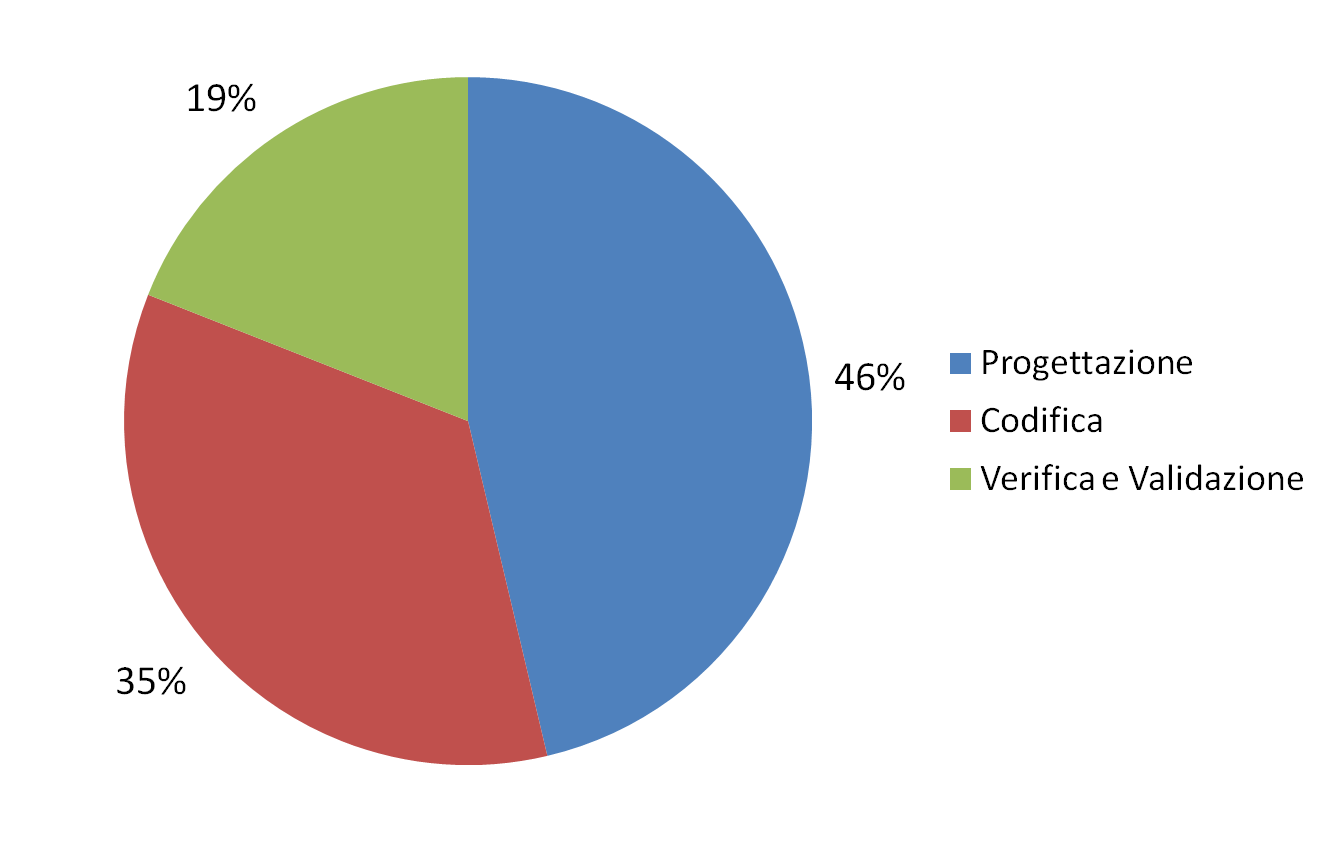
\includegraphics[scale=0.6]{../Images/pie_chart-Preventivo_Fasi}
		\caption{Incidenza Fasi di progetto}
	\end{figure}
	\pagebreak
	\subsubsection{Incidenza Ruoli}
	La figura seguente riassume velocemente il peso di ciascun ruolo riguardo la durata dell'intero progetto. Le attività di spicco sono la progettazione e la verifica.
	\begin{figure}[h!]
		\centering
		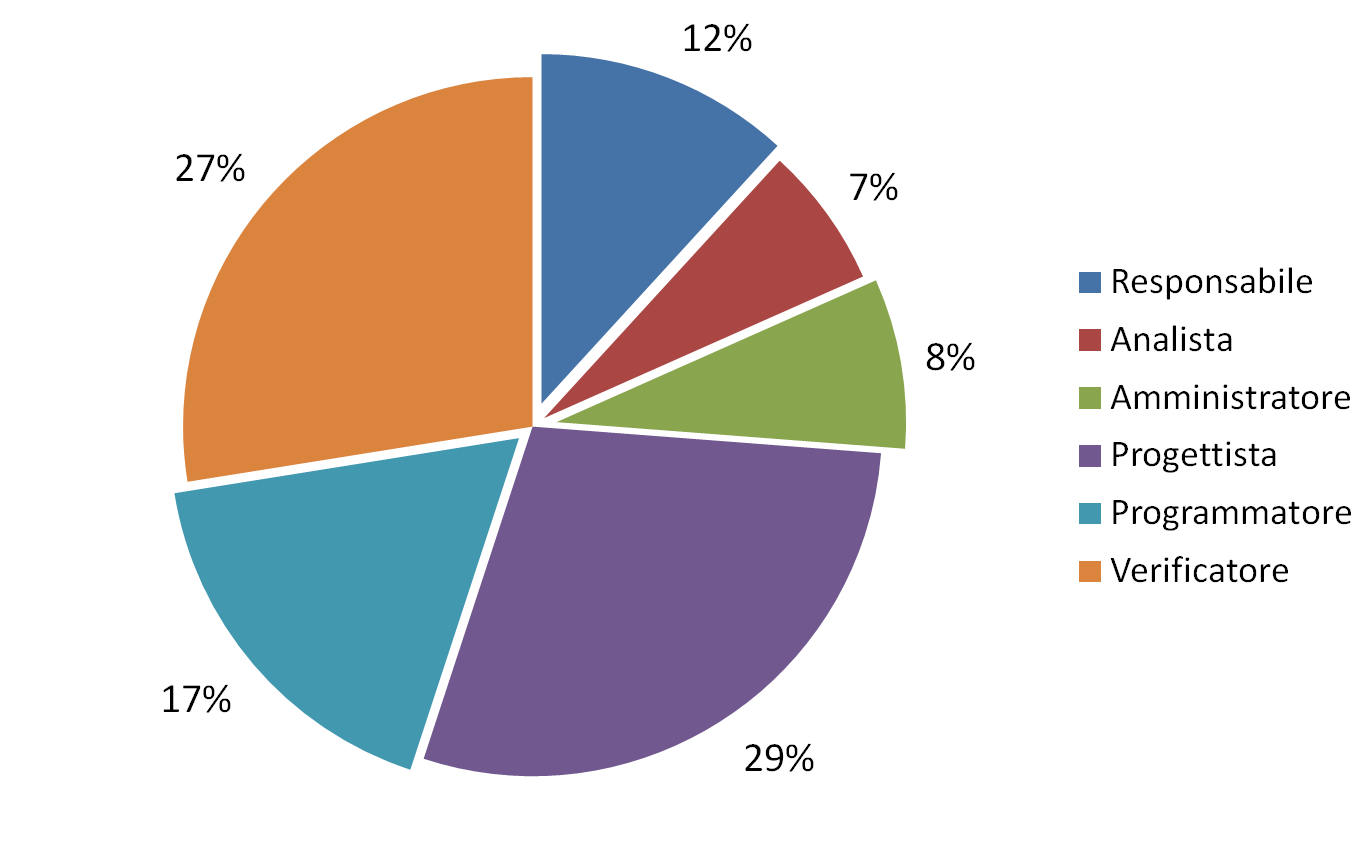
\includegraphics[scale=0.6]{../Images/pie_chart-Preventivo_Ruoli}
		\caption{Incidenza Ruoli nel progetto}
	\end{figure}
	\newpage
	\subsection{Prospetto Orario}
	Secondo quanto riportato nella sezione Vincoli, le ore di lavoro per persona devono situarsi tra un minimo di 85 e un massimo di 105. Il prospetto orario che rispecchia la pianificazione precedentemente presentata è il seguente:
	\begin{table}[h!]
		\hspace{0.6cm}\begin{tabular}{l c c c c c c}
		 	& \textbf{Davide} & \textbf{Martin} & \textbf{Marco} & \textbf{Alex} & \textbf{Luca} & \textbf{Andrea}\\
			 & \textbf{Bortot} & \textbf{V.Mbouenda} & \textbf{Crivellaro} & \textbf{Beccaro} & \textbf{Alessio} & \textbf{Multineddu}\\
			\midrule
			Responsabile 	& 10 & 5  & 10  & 5  & 10 & 5 \\
			Analista 		& 5  & 5  & 5   & 5  & 5  & 5 \\
			Amministratore 	& 5  & 10 & 5   & 10 & 5  & 10\\
			Progettista 	& 23 & 26 & 20  & 25 & 28 & 28\\
			Programmatore 	& 25 & 18 & 23  & 20 & 25 & 22\\
			Verificatore 	& 35 & 34 & 40  & 38 & 30 & 33\\
			\midrule
			\textbf{Totale} & \textbf{103} & \textbf{98} & \textbf{103} & \textbf{103} & \textbf{103} & \textbf{103}
		\end{tabular}
	\caption{Prospetto Orario}
	\end{table}
	
	Si è deciso di assegnare qualche ora di lavoro in meno a Martin Vadice Mbouenda, che è studente lavoratore e, in quanto tale, è normale possa dedicare meno tempo al presente progetto.
	
\end{document}